\documentclass[12pt]{article}
\usepackage[utf8]{inputenc}
\usepackage{float}
\usepackage{amsmath}
\usepackage{enumitem}
\usepackage[justification=centering]{caption}

\usepackage[hmargin=3cm,vmargin=6.0cm]{geometry}
%\topmargin=0cm
\topmargin=-2cm
\addtolength{\textheight}{6.5cm}
\addtolength{\textwidth}{2.0cm}
%\setlength{\leftmargin}{-5cm}
\setlength{\oddsidemargin}{0.0cm}
\setlength{\evensidemargin}{0.0cm}

%misc libraries goes here
\usepackage{tikz}
\usetikzlibrary{automata, positioning}
\newtheorem{defn}{Definition}

\begin{document}

\section*{Student Information } 
%Write your full name and id number between the colon and newline
%Put one empty space character after colon and before newline
Full Name : Beyazit Yalcinkaya  \\
Id Number : 2172138  \\

% Write your answers below the section tags
\section*{Answer 1}

\subsection*{a.} 

A 2-Dimensional Turing Machine (2D-TM) is a 7-tuple, $M = (Q, \Sigma, \Gamma, \delta, q_0, q_{accept}, q_{reject})$, where $Q$, $\Sigma$, and $\Gamma$ are all finite sets and

\begin{enumerate}
	\item $Q$ is the set of states,
	\item $\Sigma$ is the input alphabet not containing the \emph{blank symbol} $\sqcup$,
	\item $\Gamma$ is the tape alphabet, where $\sqcup \in \Gamma$ and $\Sigma \subseteq \Gamma$,
	\item $\delta: Q \times \Gamma \rightarrow Q \times \Gamma \times \{U, D, L, R\}$ is the transition function,
	\item $q_0 \in Q$ is the start state,
	\item $q_{accept} \in Q$ is the accept state, and
	\item $q_{reject} \in Q$ is the reject state, where $q_{accept} \neq q_{reject}$.
\end{enumerate}

A 2D-TM has a two dimensional infinite tape. Upper left corner of the tape is the first cell. Tape goes to infinity towards right and down. A 2D-TM $M = (Q, \Sigma, \Gamma, \delta, q_0, q_{accept}, q_{reject})$ receives its input $w = w_1 w_2 \ldots w_n \in \Sigma^*$ on the first line of the 2D input tape, i.e., $w_1$ is on the upper left corner of the tape and the leftmost $n$ squares of the first line is occupied. Since the input language does not contain $\sqcup$, the first blank appearing on the first line marks the end of the input.

A \emph{configuration} of 2D-TM is represented as follows
%\[\left(q, [i, j], \langle w_1 w_2 \ldots w_m \rangle, \langle w_{m+1} w_{m+2} \ldots w_{2m} \rangle, \ldots, \langle w_{(n -1)m + 1} w_{(n-1)m + 2} \ldots w_{nm} \rangle\right),\]
\[\left(q, [i, j], \Psi = \{ \langle[k, l], w_{kl} \rangle \mid  k, l \in Z^{+} \land w_{kl} \in \Gamma \land ((k = i \land l = j) \lor w_{kl} \neq \sqcup) \} \right),\]
where $q \in Q$ is the current state, $[i, j]$ is the index of the position of the read/write head where $i$ and $j$ are positive integers indicating row and column number of the head, respectively, and, $\Psi = \{ \langle[k, l], w_{kl} \rangle \mid  k, l \in Z^{+} \land w_{kl} \in \Gamma \land ((k = i \land l = j) \lor w_{kl} \neq \sqcup) \}$ is the finite set of all cells with non-blank entries and the cell under the read/write head. Note that, upper left corner of the input tape is indexed by $[1, 1]$, i.e., for $[k, l]$, $k$ increases towards down and $l$ increases towards right.

Now, we formalize how 2D-TM \emph{computes}. Say that configuration $C_1$ \emph{yields} configuration $C_2$ if the 2D-TM can legally go from $C_1$ to $C_2$ in a single step. Suppose $q, \tilde{q} \in Q$, $i, j \in Z^{+}$, and $w_{ij}, \tilde{w_{ij}}, w_{(i-1)j}, w_{(i+1)j}, w_{i(j-1)}, w_{i(j+1)} \in \Gamma$. We formalize the notion of computation as follows.

\

\begin{enumerate}
	\item For $\delta(q, w_{ij}) = (\tilde{q}, \tilde{w_{ij}}, U)$, \[\left(q, [i, j], \Psi \right) \text{ yields } \left(\tilde{q}, [i-1, j], \tilde{\Psi} \right),\]
where $\langle [i, j], w_{ij} \rangle \in \Psi$ and $\langle [i-1, j], w_{(i-1)j} \rangle \in \Psi$ if $w_{(i-1)j} \neq \sqcup$, else $\langle [i-1, j], w_{(i-1)j} \rangle \not \in \Psi$; and $\langle [i-1, j], w_{(i-1)j} \rangle \in \tilde{\Psi}$ and $\langle [i, j], \tilde{w_{ij}} \rangle \in \tilde{\Psi}$ if $\tilde{w_{ij}} \neq \sqcup$, else $\langle [i, j], \tilde{w_{ij}} \rangle \not \in \tilde{\Psi}$.
	\item For $\delta(q, w_{ij}) = (\tilde{q}, \tilde{w_{ij}}, D)$, \[\left(q, [i, j], \Psi \right) \text{ yields } \left(\tilde{q}, [i+1, j], \tilde{\Psi} \right),\]
where $\langle [i, j], w_{ij} \rangle \in \Psi$ and $\langle [i+1, j], w_{(i+1)j} \rangle \in \Psi$ if $w_{(i+1)j} \neq \sqcup$, else $\langle [i+1, j], w_{(i+1)j} \rangle \not \in \Psi$; and $\langle [i+1, j], w_{(i+1)j} \rangle \in \tilde{\Psi}$ and $\langle [i, j], \tilde{w_{ij}} \rangle \in \tilde{\Psi}$ if $\tilde{w_{ij}} \neq \sqcup$, else $\langle [i, j], \tilde{w_{ij}} \rangle \not \in \tilde{\Psi}$.
	\item For $\delta(q, w_{ij}) = (\tilde{q}, \tilde{w_{ij}}, L)$, \[\left(q, [i, j], \Psi \right) \text{ yields } \left(\tilde{q}, [i, j-1], \tilde{\Psi} \right),\]
where $\langle [i, j], w_{ij} \rangle \in \Psi$ and $\langle [i, j-1], w_{i(j-1)} \rangle \in \Psi$ if $w_{i(j-1)} \neq \sqcup$, else $\langle [i, j-1], w_{i(j-1)} \rangle \not \in \Psi$; and $\langle [i, j-1], w_{i(j-1)} \rangle \in \tilde{\Psi}$ and $\langle [i, j], \tilde{w_{ij}} \rangle \in \tilde{\Psi}$ if $\tilde{w_{ij}} \neq \sqcup$, else $\langle [i, j], \tilde{w_{ij}} \rangle \not \in \tilde{\Psi}$.
	\item For $\delta(q, w_{ij}) = (\tilde{q}, \tilde{w_{ij}}, R)$, \[\left(q, [i, j], \Psi \right) \text{ yields } \left(\tilde{q}, [i, j+1], \tilde{\Psi} \right),\]
where $\langle [i, j], w_{ij} \rangle \in \Psi$ and $\langle [i, j+1], w_{i(j+1)} \rangle \in \Psi$ if $w_{i(j+1)} \neq \sqcup$, else $\langle [i, j+1], w_{i(j+1)} \rangle \not \in \Psi$; and $\langle [i, j+1], w_{i(j+1)} \rangle \in \tilde{\Psi}$ and $\langle [i, j], \tilde{w_{ij}} \rangle \in \tilde{\Psi}$ if $\tilde{w_{ij}} \neq \sqcup$, else $\langle [i, j], \tilde{w_{ij}} \rangle \not \in \tilde{\Psi}$.
\end{enumerate}

Special cases occur when the head is on the leftmost or on the upmost cells of the tape. For a configuration with head index $[i, j]$, if $i$ is equal to $1$, i.e., head is on the upmost cells, an up-moving transition does not change the index of the head, i.e., head stays on $[i, j]$. If $j$ is equal to $1$, i.e., head is on the leftmost cells, a left-moving transition does not change the index of the head.

For 2D-TM $M = (Q, \Sigma, \Gamma, \delta, q_0, q_{accept}, q_{reject})$ on input $w = w_1w_2\ldots w_n$, \emph{start configuration} is
\[\left(q_0, [1, 1], \{ \langle [1,1], w_1 \rangle, \langle [1,2], w_2 \rangle, \ldots, \langle [1,n], w_n \rangle \} \right).\]
In an \emph{accepting configuration}, the state of the configuration is $q_{accept}$. In a \emph{rejecting configuration}, the state of the configuration is $q_{reject}$. Accepting and rejecting configurations are halting configurations and do not yield further configurations. A 2D-TM $M$ accepts input $w$ if a sequence of configurations $C_1, C_2, \ldots, C_k$ exists, where (i) $C_1$ is the start configuration of $M$ on input $w$, (ii) each $C_i$ yields $C_{i+1}$, and (iii) $C_k$ is an accepting configuration.

We say that a 2D-TM $M$ decides a language $L$ if for all $w \in L$, $M$ accepts $w$ and for all $\tilde{w} \not \in L$, $M$ rejects $\tilde{w}$. $M$ is called a decider for the language $L$ and $L$ is called a decidable language.


%$1 \leq i \leq n$ and $1 \leq j \leq m$
\
\subsection*{b.}

First, let us give the intuition behind the proof of equivalence between 2D-TM and TM. Definition of the machines and transition functions are very similar. We will only show the equivalence between the 2D and 1D infinite tapes. The equivalence directly comes from the Cantor pairing function, i.e., $\pi(i, j) := \frac{1}{2}(i + j)(i + j + 1) + i$, where $[i, j]$ is the row-column indexing. Notice that, here, indexing of rows and columns start from zero, i.e., index of the upper left corner is $[0, 0]$.

In the problem, it is given that on an input with length $n$, 2D-TM takes $t$ steps. Assuming input processing is separated from these $t$ steps, total number of steps taken is $n + t$. In the previous part, it is stated that input is given to 2D-TM on the first line of the input tape. Then, the index of the last character of the input is $[0, n - 1]$. After applying Cantor pairing function to map the input tapes of 2D-TM and TM, we get $\pi(0, n - 1) = \frac{n^2 - n}{2}$. That is, it takes $\frac{n^2 - n}{2}$ steps to process the input. $t$ steps taken by 2D-TM is basically the Manhattan distance on the input tape, i.e., $t$ is the summation of horizontal and vertical moves on the tape. For a safe analysis, we will assume the worst, i.e., $t$ consists of only vertical moves. Then. the furthest cell reached by the machine is $[t, 0]$, which takes $\pi(t, 0) = \frac{t^2+3t}{2}$ steps on a TM. Therefore, the same computation takes $\frac{n^2 - n}{2} + \frac{t^2+3t}{2}$ steps on a standard TM, i.e., $O(n^2 + t^2)$.

\subsection*{c.} 

Notice that for the sake of simplicity, we avoid unnecessary transitions on the given 2D-TM below. The basic idea behind the machine is that it basically scans the input tape along its diagonals. For this purposes it uses $x$ and $y$ symbols for marking. The graphical description is given below.

\begin{center}
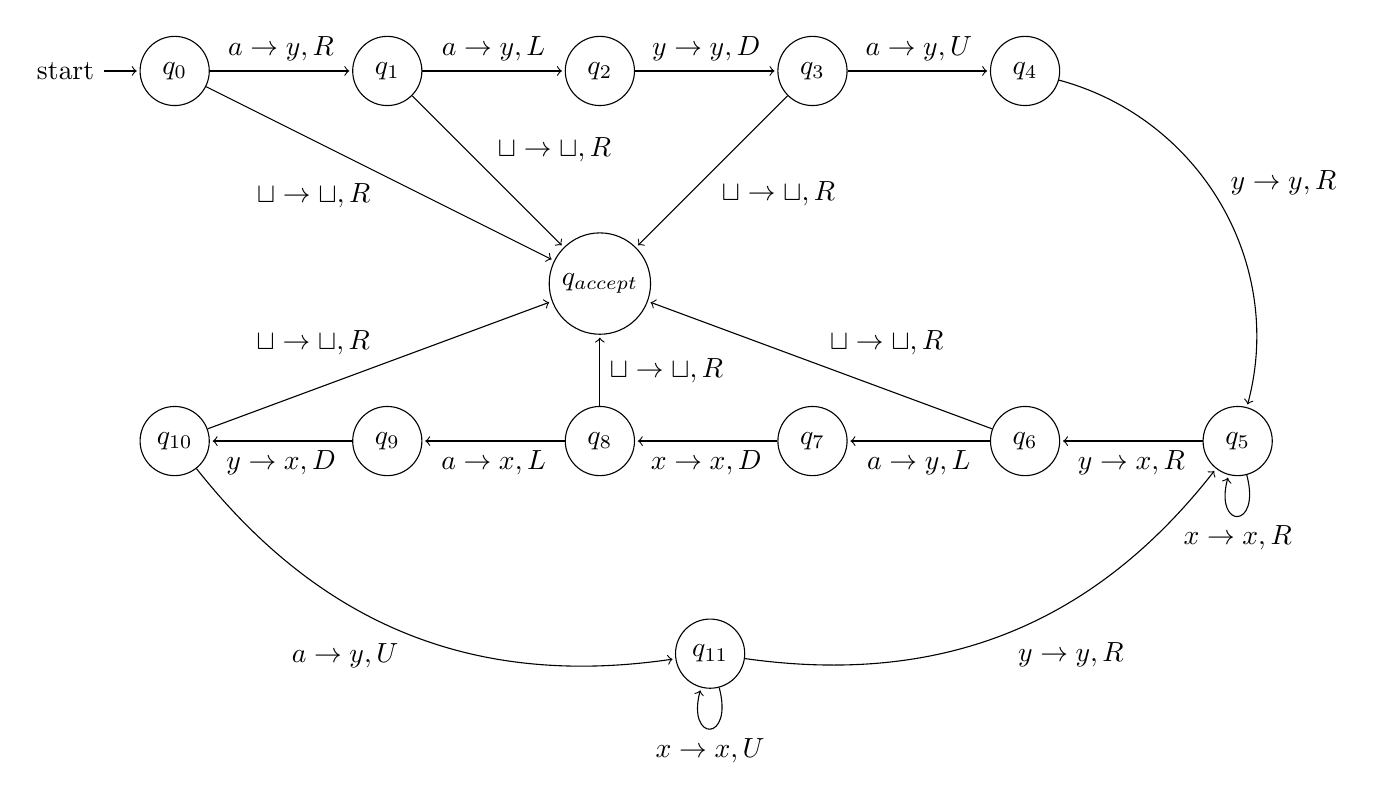
\begin{tikzpicture}[shorten >=1pt,node distance=2.7cm,on grid,auto]
             \node[state,initial] (q_0) {$q_0$};
             \node[state] (q_1) [right=of q_0] {$q_1$};
             \node[state] (q_2) [right=of q_1] {$q_2$};
             \node[state] (q_3) [right=of q_2] {$q_3$};
             \node[state] (q_4) [right=of q_3] {$q_4$};
             \node[state] (q_6) [below=of q_4, yshift=-2cm] {$q_6$};
             \node[state] (q_5) [right=of q_6] {$q_5$};
             \node[state] (q_7) [left=of q_6] {$q_7$};
             \node[state] (q_8) [left=of q_7] {$q_8$};
             \node[state] (q_9) [left=of q_8] {$q_9$};
             \node[state] (q_{10}) [left=of q_9] {$q_{10}$};
             \node[state] (q_{11}) [below=of q_8, xshift=1.4cm] {$q_{11}$};
             \node[state] (q_{accept}) [below=of q_2] {$q_{accept}$};
             \path[->]
             (q_0) edge node {$a \rightarrow y, R$} (q_1)
             (q_0) edge node[swap] {$\sqcup \rightarrow \sqcup, R$} (q_{accept})
             (q_1) edge node {$\sqcup \rightarrow \sqcup, R$} (q_{accept})
             (q_3) edge node {$\sqcup \rightarrow \sqcup, R$} (q_{accept})
             (q_6) edge node[swap] {$\sqcup \rightarrow \sqcup, R$} (q_{accept})
             (q_8) edge node[swap] {$\sqcup \rightarrow \sqcup, R$} (q_{accept})
             (q_{10}) edge node {$\sqcup \rightarrow \sqcup, R$} (q_{accept})
             (q_1) edge node {$a \rightarrow y, L$} (q_2)
             (q_2) edge node {$y \rightarrow y, D$} (q_3)
             (q_3) edge node {$a \rightarrow y, U$} (q_4)
             (q_4) edge[bend left=45] node {$y \rightarrow y, R$} (q_5)
             (q_5) edge[loop below] node [swap] {$x \rightarrow x, R$} (q_5)
             (q_5) edge node {$y \rightarrow x, R$} (q_6)
             (q_6) edge node {$a \rightarrow y, L$} (q_7)
             (q_7) edge node {$x \rightarrow x, D$} (q_8)
             (q_8) edge node {$a \rightarrow x, L$} (q_9)
             (q_9) edge node {$y \rightarrow x, D$} (q_{10})
             (q_{10}) edge[bend right=30] node [swap] {$a \rightarrow y, U$} (q_{11})
             (q_{11}) edge[loop below] node [swap] {$x \rightarrow x, U$} (q_11)
             (q_{11}) edge[bend right=30] node [swap] {$y \rightarrow y, R$} (q_5);
\end{tikzpicture}
\end{center}


\section*{Answer 2} 

\subsection*{a.} 

Let $L_A$ and $L_B$ be two decidable languages. Then, there exist a decider $M_A$ for $L_A$ and a decider $M_B$ for $L_B$. To prove that the set of decidable languages are closed under concatenation, we give a definition of the TM $M$ deciding strings of the form $w = w_A w_B$, where $w_A \in L_A$ and $w_B \in L_B$.

$M \ =$ ``On input $w$, where $w = w_A w_B$, $w_A \in L_A$, and $w_B \in L_B$:
\begin{enumerate}[leftmargin=2.50cm]
	\item Nondeterministically split $w$ into two substrings: $w_A$ and $w_B$.
	\item Run $M_A$ on the input $w_A$.
	\item If $M_A$ rejects $w_A$, then \texttt{REJECT}.
	\item Run $M_B$ on the input $w_B$.
	\item If $M_B$ rejects $w_B$, then \texttt{REJECT}.
	\item \texttt{ACCEPT}."
\end{enumerate}

Notice that, $M$ is a nondeterministic TM (NTM). Since it has been shown that NTM is equivalent to TM, there exists a TM equivalent to $M$. Therefore, $M$ is a decider for concatenated strings of two decidable languages, i.e., the set of decidable languages are closed under concatenation.



\subsection*{b.}

Let $L$ a recognizable language. Then, there exists a recognizaer $M$ for $L$. To prove that the set of decidable languages are closed under concatenation, we give a definition of the TM $M'$ recognizing strings $w \in L^*$.

$M' \ =$ ``On input $w$, where $w \in L^*$:
\begin{enumerate}[leftmargin=2.50cm]
	\item Nondeterministically choose a number $k$ and split $w$ into $k$ substrings: $w = w_1\ldots w_k$.
	\item For $i = 1\ldots k$, run $M$ on each $w_i$ in parallel.
	\item If $M$ accepts all $w_i$, then \texttt{ACCEPT}.
	\item \texttt{REJECT}."
\end{enumerate}

Notice that, $M'$ is a nondeterministic TM (NTM). Since it has been shown that NTM is equivalent to TM, there exists a TM equivalent to $M'$. Therefore, $M'$ is a recognizer for Kleene star of recognizable languages, i.e., the collection of recognizable languages are closed under star.

\subsection*{c.} 

Let $L$ be an infinite recursively enumerable language. In the textbook of the course, Theorem 3.21 states that a language is Turing-recognizable if and only if some enumerator enumerates it. Related proof is given in the book. Then, there exists an enumerator $E$ that enumerates all $w \in L$, i.e., $L(E) = L$. Now, let us construct a new enumerator $E'$ defined as follows.

$E' \ =$ ``On input $\langle E \rangle$, where $E$ is an enumerator of a recognizable language:
\begin{enumerate}[leftmargin=2.50cm]
	\item Simulate $E$ and let it print a string.
	\item If no string is outputted yet or the printed string lexicographically comes later than the last outputted string, then output the printed string.
	\item Go to 1."
\end{enumerate}

Trivially, $L' = L(E') \subseteq L(E) = L$. $E'$ enumerates an infinite decidable language. Now, let us prove this. Let $M'$ be the decider for the language enumerated by $E'$ defined as follows.

$M' \ =$ ``On input $\langle E', w \rangle$, where $w \in L(E')$:
\begin{enumerate}[leftmargin=2.50cm]
	\item Simulate $E'$ and let it print a string.
	\item If printed string is equal to $w$, then \texttt{ACCEPT}.
	\item If printed string lexicographically comes later than $w$, then \texttt{REJECT}.
	\item Go to 1."
\end{enumerate}

$M'$ is a decider for $L'$ and $L' \subseteq L$. Therefore, we showed by construction that every infinite recursively enumerable language has an infinite decidable subset.

\section*{Answer 3}

\subsection*{a.} 

NFA is equivalent to DFA and DFA decides regular expressions; hence, both $L(A)$ and $L(B)$ are regular expressions. Notice that, $L(A) \subseteq L(B)$ implies $L(A) \cap \overline{L(B)} = \emptyset$. To prove decidability of $SUBS$, we will construct a new DFA $C$, language of which is $L(C) = L(A) \cap \overline{L(B)}$. Since regular expressions are closed under complementation and intersection, $L(C)$ is also a regular expression. Then, there exists a DFA $C$ deciding $L(C)$. Now, we will define a decider for $SUBS$. Call this decider TM $M$. Basically, $M$ will construct a new DFA $C$ and check $L(C) = \emptyset$.


$M \ =$ ``On input $\langle A, B \rangle$, where $A$ is a DFA, $B$ is an NFA, and $L(A) \subseteq L(B)$:
\begin{enumerate}[leftmargin=2.50cm]
	\item Construct a new DFA $C$ as described.
	\item Mart start state of $C$.
	\item Repeat until no new states get marked: Mark any state that has a transition coming into it from any state that is already marked.
	\item If no accept state is marked, \texttt{ACCEPT}; otherwise, \texttt{REJECT}.”
\end{enumerate}


\subsection*{b.}

To prove the decidability of $E$, we will define a context-free language $B$ as follows.
\[B =\{w \mid w \text{ has more 1s than 0s}\}\]
We can construct a new machine $A$, where $L(A) = B \cap L(M)$. Note that, since $B$ is CFL and $L(M)$ is RE $A$ is a PDA. Then, there exists a CFG $G$, where $L(G) = L(A)$. If $L(G) \neq \emptyset$, then $M$ accepts some string with more 1s than 0s. Using this notion, we can define a decider $D$ for $E$.

$D \ =$ ``On input $\langle M \rangle$, where $M$ is a DFA that accepts some string with more 1s than 0s:
\begin{enumerate}[leftmargin=2.50cm]
	\item Construct CFG $G$ as described.
	\item Mark all terminal symbols in $G$.
	\item Repeat until no new variables get marked: Mark any variable $A$ where $G$ has a rule $A\rightarrow U_1U_2\ldots U_k$ and each symbol $U_1, U_2 , \ldots U_k$ has already been marked.
	\item If the start variable is not marked, \texttt{REJECT}; otherwise, \texttt{ACCEPT}.”
\end{enumerate}

\section*{Answer 4}

The problem is formulated by the language below.
\[
L = \{ \langle M_1, M_2 \rangle \mid M_1 \text{ and } M_2 \text{ are 2D finite automaton and } L(M_1) = L(M_2)\}
\]
Now, we prove that $L$ is undecidable. First obverse that, 2D-DFA is equivalent to LBA. The reasoning behind this observation is as follows. Since LBA has finitely many configurations, a 2D-DFA can capture these finitely many configurations on its states. That is, although, a 2D-DFA cannot write anything on the tape, it can capture the same writing behaviour on its states due to its finite nature just like LBA. A direct mapping from LBA to 2D-DFA can be defined as follows.

\begin{enumerate}
	\item Map input tape of LBA to the new 2D-DFA by adding delimiter symbols left, right, up and down of the input string.
	\item Map every possible configuration to a state in 2D-DFA, i.e., define $k|Q||\Sigma|^{k}$ many states in the new 2D-DFA, where $k$ is the length of the input.
	\item Using configuration-state mappings, translate transition function of LBA to 2D-DFA.
\end{enumerate}

Let us define a new language.
\[
E_{2D-DFA} = \{\langle M \rangle \mid M \text{ is a 2D-DFA and } L(M) = \emptyset\}
\]
We first prove that $E_{2D-DFA}$ is undecidable. Notice that, in the textbook Theorem 5.10 proves that $E_{LBA}$ is undecidable. Assume $A$ decides $E_{2D-DFA}$. Then, we construct $B$ to decide $E_{LBA}$.


$B \ =$ ``On input $\langle M \rangle$, where $M$ is a LBA and $L(M) = \emptyset$:
\begin{enumerate}[leftmargin=2.50cm]
	\item Construct 2D-DFA $M'$ as described.
	\item Run $A$ on $M'$.
	\item If $A$ rejects, \texttt{REJECT}; if $A$ accepts, \texttt{ACCEPT}.”
\end{enumerate}

It has been prove by Theorem 5.10 in the textbook that $E_{LBA}$ is undecidable. Existence of $B$ leads to a contradiction. Therefore, $E_{2D-DFA}$ is undecidable. Now, we are ready to prove undecidability of $L$. Assume $L$ is decidable and $C$ decides $L$. We construct $D$ to decide $E_{2D-DFA}$.

$D \ =$ ``On input $\langle M \rangle$, where $M$ is a 2D-DFA and $L(M) = \emptyset$:
\begin{enumerate}[leftmargin=2.50cm]
	\item Run $C$ on $\langle M, \tilde{M} \rangle$, where $\tilde{M}$ is a 2D-DFA that rejects all inputs.
	\item If $C$ rejects, \texttt{REJECT}; if $C$ accepts, \texttt{ACCEPT}.”
\end{enumerate}

Since we have already proved that $E_{2D-DFA}$ is undecidable, existence of $D$ leads to a contradiction. Therefore, $L$ is undecidable.

\section*{BONUS 1}

The observable universe is limited. The number of atoms in the observable universe, let us call this number $\aleph$, must also be limited since observable universe defines a limited spherical volume.

We provide a counter example to show that Powerpoint slide editing program is not as powerful as a Turing Machine.

Let $L$ be a language defined as follows and $M$ be a decider for $L$ with input alphabet $\Sigma$.

\[
L = \{w \mid w \in \Sigma^* \text{ and length of } w \text{ is } \aleph + 1\}
\]

Such an $M$, indeed, exists. It is just a TM counting number of symbols of the input and at the end it compares this number with $\aleph + 1$. If the count is equal, then it accepts, else rejects. However, a Powerpoint slide deciding $L$ cannot exists because even if we use all the atoms in the universe to construct a machine for Powerpoint, the input tape would not be enough to encode members of the language.

Notice that, Powerpoint is defined is a slideshow presentation program by its creator. A program is defined as a collection of instructions that can be executed by a computer to perform a specific task. Therefore, Powerpoint is a physically entity that can only operate on another physical entity, i.e., it is not an abstract concept or a set of semantically defined operations. This observations means that we cannot talk about Powerpoint program being as powerful as a TM because it does not have a formal definition which consists of a set of entities and operations on these entities defining a computational model. Reader might think that Powerpoint program is similar to programming languages and therefore, Powerpoint might be equivalent to TM. However, programming languages are formally defined models for computation. Basically a programming language is a set of strings defined by a formal grammar and their corresponding semantic operations. Therefore, a programming language, by itself, does not set any boundary and it is an abstract definition. The boundaries (such as maximum values for integer variables) are set by the execution platform, not by the language itself. In conclusion, programming languages are, indeed, Turing-complete but they are surely different from Powerpoint slide editing program.
\end{document}

​